\begin{figure}[h!]
\centering
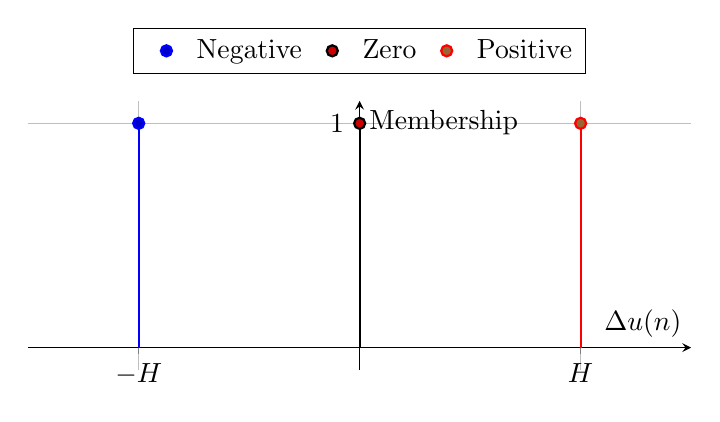
\begin{tikzpicture}
\begin{axis}[
    axis lines=middle,
    xlabel={$\Delta u(n)$},
    ylabel={Membership},
    ymin=-0.1, ymax=1.1,
    xmin=-15, xmax=15,
    xtick={-10, 0, 10},
    xticklabels={$-H$, $0$, $H$},
    ytick={0, 1},
    grid=both,
    width=10cm, height=5cm,
    legend style={at={(0.5,1.1)}, anchor=south, legend columns=-1}
]

% Singleton at -H (Negative)
\addplot+[ycomb, thick, blue, mark=*] coordinates {(-10,1)};
\addlegendentry{Negative}

% Singleton at 0 (Zero)
\addplot+[ycomb, thick, black, mark=*] coordinates {(0,1)};
\addlegendentry{Zero}

% Singleton at +H (Positive)
\addplot+[ycomb, thick, red, mark=*] coordinates {(10,1)};
\addlegendentry{Positive}

\end{axis}
\end{tikzpicture}
\caption{Output fuzzy sets as singleton values at $-H$, $0$, and $H$}
\label{fig:fig2}
\end{figure}